\section{What is a First-Order Polynomial?}

A \textbf{first-order polynomial} is a polynomial of degree 1. It has the general form:
\[
y = mx + b
\]
where:
\begin{itemize}
    \item \( m \) is the slope of the line, which indicates how steep the line is.
    \item \( b \) is the y-intercept, which is the point where the line crosses the y-axis.
\end{itemize}

The graph of a first-order polynomial is a straight line.

\clearpage
\subsection{Python Code Example}

Here is a Python code snippet to plot a first-order polynomial using Matplotlib:

\begin{lstlisting}[language=Python, caption=Python code to plot a first-order polynomial]
import matplotlib.pyplot as plt

def first_order_polynomial(X: list[int], a: float, b: float) -> list[float]:

    Y: list[float] = []
    for x in X:
        y = a * x + b
        Y.append(y)

    return Y


x = list(range(-10, 10))
y = first_order_polynomial(x, 2, -2)

plt.plot(x, y, "-o", label="Line")
plt.title("First Order Polynomial")
plt.xlabel("x")
plt.ylabel("y")
plt.grid(True)
plt.show()
\end{lstlisting}

\section{Visualization}

Below is the plot of the first-order polynomial generated by the Python code:

\begin{figure}[t]
\centering
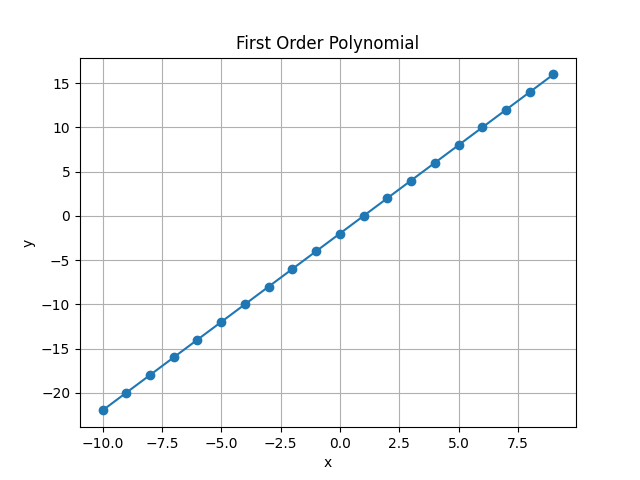
\includegraphics[width=0.8\textwidth]{PART3/1_polynomials/line.png}
\caption{Plot of the first-order polynomial $y = 2x - 2$.}
\end{figure}
